\documentclass{article}
\usepackage[utf8]{inputenc}
\usepackage[a4paper, total={6in, 8in}]{geometry}
\usepackage{indentfirst}
\usepackage{authblk}
\usepackage{graphicx}
\usepackage{hyperref}

%\usepackage[square,numbers]{natbib}
%\usepackage[square,sort,comma,numbers]{natbib}
\usepackage[style=numeric]{biblatex}
\addbibresource{references.bib}
\usepackage[dvipsnames]{xcolor}

\usepackage{amsmath}
\usepackage{amsthm} % proof environment
\usepackage{amsfonts}
\usepackage{amssymb}

\usepackage{caption}
\usepackage[shortlabels]{enumitem}
\usepackage{float}
\usepackage{listings}
\usepackage{soul} % highlighting

\newcommand{\floor}[1]{\left\lfloor #1 \right\rfloor}
\newcommand{\ceil}[1]{\left\lceil #1 \right\rceil}

\hypersetup{
  colorlinks=true,
  linkcolor=blue,
  filecolor=blue,
  urlcolor=blue,
  citecolor=OliveGreen
}
\urlstyle{same}
\setlength{\parindent}{2em}
\setlength{\parskip}{1ex}
\captionsetup[figure]{labelfont={bf},name={Fig.},labelsep=period}
\numberwithin{figure}{section}

\title{\huge{\textbf{Zarcanum: A Proof-of-Stake Scheme for Confidential Transactions with Hidden Amounts}}}

\author{\large{sowle}\textsuperscript{1}, \large{koe}\textsuperscript{2}}
\affil{\small{
    \textsuperscript{1}Zano project, \texttt{val@zano.org} \\
    \textsuperscript{2}Independent researcher, \texttt{ukoe@protonmail.com}
}}

\date{\small{October 2021\footnote{Version 4.3. Last update: 2021-10-06. Check \href{https://github.com/hyle-team/docs/tree/master/PoS/PoS_with_HA}{here} for the latest version.}}}


\begin{document}
\maketitle

\begin{abstract}
This article explores a Proof-of-Stake mining algorithm in an environment where amounts are hidden with homomorphic commitments, in particular, using confidential transactions. Our goal was to avoid revealing amounts and other sensitive information (like which output was used to stake a given block) to blockchain observers when doing staking.

Our contribution is a Proof-of-Stake mining scheme that does not reveal amounts and is compatible with ring confidential transactions.
\end{abstract}

\section{Notation}
Let $\mathbb{G}$ denote the main subgroup of the Ed25519 curve (\cite{ed25519_site}) and $\mathbb{Z}_p$ denote a ring of integers modulo $p$.

$l$ is the order of $\mathbb{G}$: $l = \#\mathbb{G} = 2^{252} + 27742317777372353535851937790883648493$.

For  any  set $X$, $x \stackrel{\$}{\leftarrow} X$ means uniform  sampling of $x$ at random from $X$. 

For any integers $x$, $y$, $\floor{\frac{x}{y}}$ denotes the integer part of \textit{integer arithmetic} division.


\section{Classic PoS scheme (open amounts)} \label{s_open_amounts}

\indent
In this section we describe how PoS mining was originally implemented in Zano\footnote{This scheme is based on ideas from the PeerCoin project \cite{peercoin_wp}. }.

\indent
Suppose Alice has some unspent outputs and wants to mine a PoS block using one of them as a stake. In such a scenario she acts as follows (Fig. \ref{fig:1.1}):

\begin{enumerate}
\item Gets the hash identifier of the last PoW block in the blockchain, $last\_pow\_id$.

\item Gets the last PoS block in the blockchain and gets the stake kernel hash identifier from it, $last\_pos\_kernel\_id$. Together with $last\_pow\_id$ they are called the ``stake modifier''. It changes each time a new block is added to the blockchain. 

\item Makes set $T$ of all possible timestamps for the new PoS block:
\[ T = \{t : t_{min} \leq t \leq t_{max}, \; t \equiv 0 \mod{15} \} \]
where $t_{min}$ and $t_{max}$ are bound to the current blockchain conditions. For the sake of simplicity we can assume that
\[ t_{min} = \tau - T, \; t_{max} = \tau + T \]
where $T$ is a constant and $\tau$ is the current timestamp established in such a way that it is the same across all the network's nodes.

\item Makes set $U$ of all her unspent transaction outputs (UTXO) that are eligible for staking (i.e.\ not locked, mature enough, etc.). For each output $u$ from $U$ she also precalculates the key image $I_u$.

\item Each pair $(t, u) \in T \times U$ is checked against the PoS winning condition as follows:

    \begin{enumerate}
    \item For output $u$ build \textit{stake kernel} $K_u$ as a concatenation:
    \[ K_u = last\_pow\_id \;\|\; last\_pos\_kernel\_id \;\|\; t \;\|\; I_u \]
    where $I_u$ is the key image of the stake output $u$;
    
    \item Calculate hash $h_u = cn\_fast\_hash(K_u)$\footnote{$cn\_fast\_hash$ is an alias for the Keccak-256 hash function, which is similar to SHA3-256 but differs in padding bits.};
    
    \item Finally, check the main condition:
    \begin{equation} \label{old_pos_main_cond}
    \frac{h_u D}{a_u} \stackrel{?}{\leq} 2^{256} \end{equation} 
    where $D$ is the current PoS difficulty, and $a_u$ is the amount of the stake output $u$.
    
    
    \begin{figure}[ht!]
    \centering
    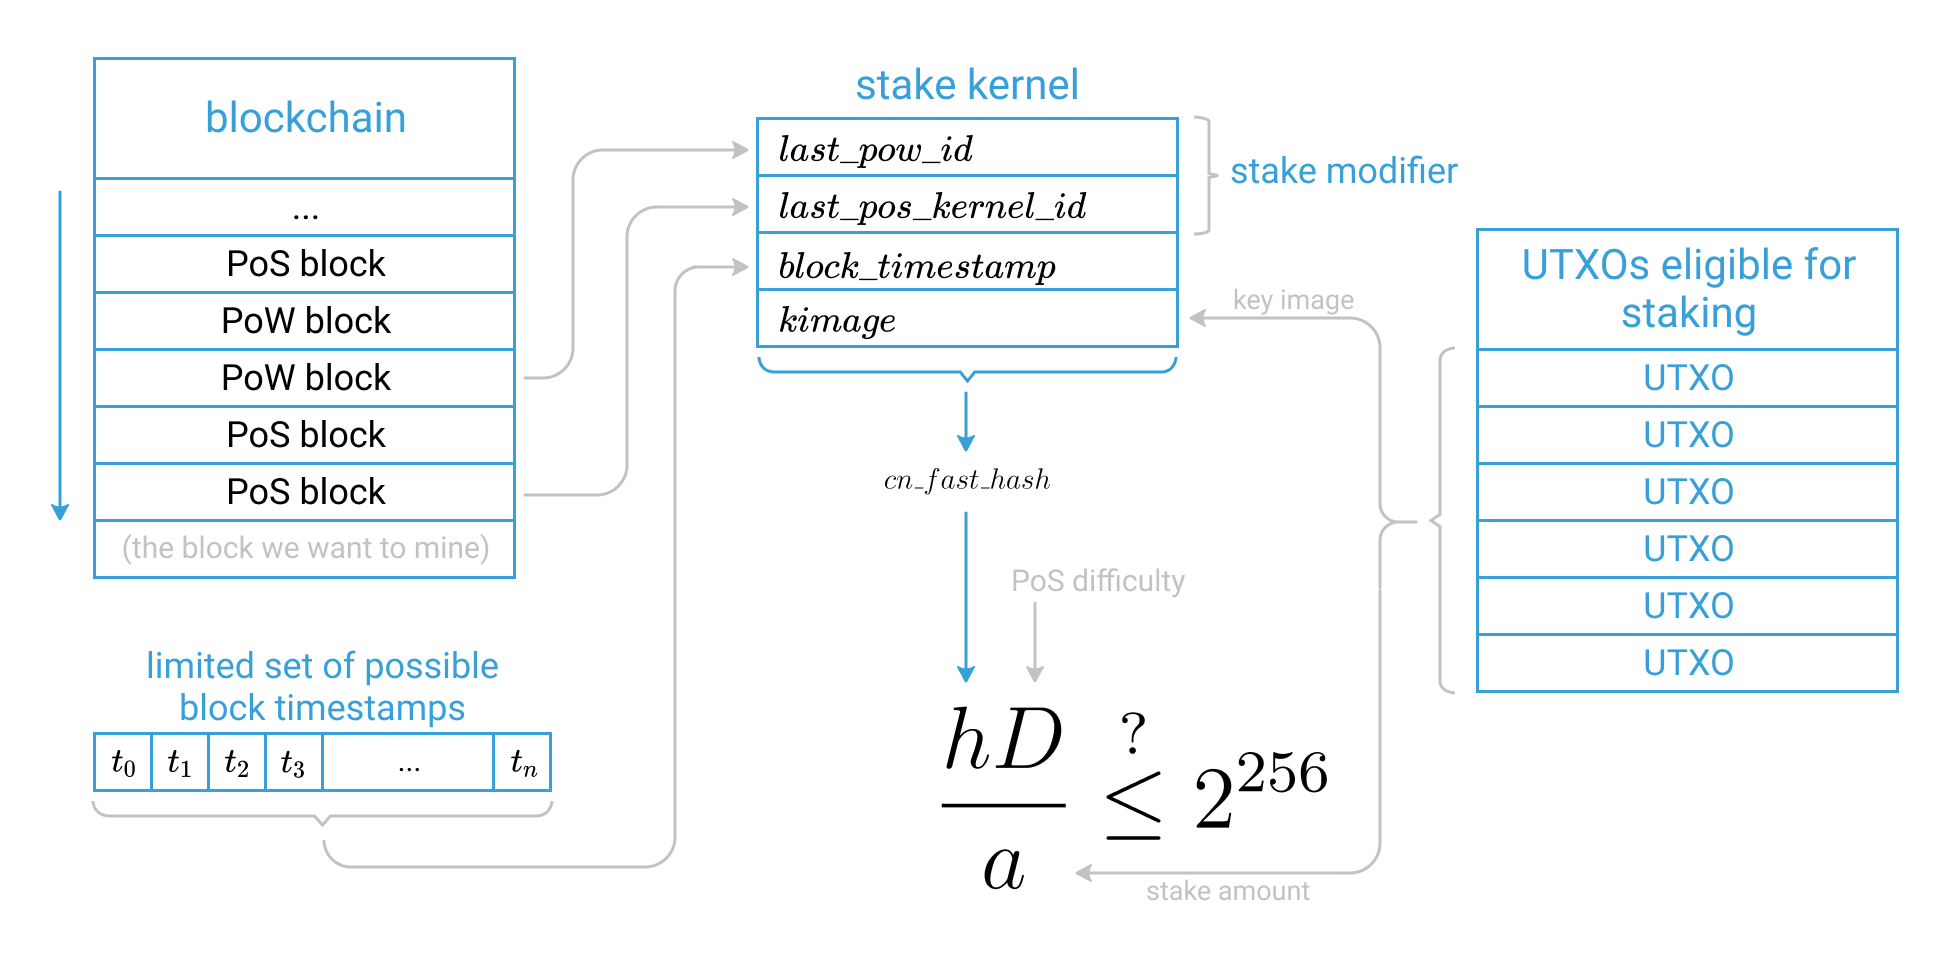
\includegraphics[scale=0.61]{fig_1.png}
    \caption{Scheme of the PoS mining process, as originally implemented in Zano}
    \label{fig:1.1}
    \end{figure}

    \end{enumerate}

    If inequality (\ref{old_pos_main_cond}) holds then it means the success of PoS mining! A block with timestamp $t$ and a stake input spending output $u$ can be constructed and broadcast to the network.
    
\end{enumerate}


If for all pairs $(t, u)$ inequality (\ref{old_pos_main_cond}) does not hold, Alice needs to wait until one of the following happens:
\begin{itemize}
    \item a new block is added to the blockchain (this will change either $last\_pow\_id$ or $last\_pos\_kernel\_id$);
    \item some time passes (this will change $t_{min}$ and $t_{max}$).
\end{itemize}

\indent
Once this happens, Alice can attempt mining again (items 1-5), as all $K_u$, and thus $h_u$, will have different values, giving new opportunities to meet the main condition.

We'd like to note the following important property of (\ref{old_pos_main_cond}): as $h_u$ is the result of a cryptographic hash function and can be considered as distributed evenly over the interval $[0, 2^{256})$, the probability of meeting the main condition is proportional to output amount $a_u$. 

%\newpage

\section{Hidden amounts: the problem and the solution} \label{sec_basic_idea}

Consider a hidden amount scheme\footnote{E.g., Confidential Transactions (CT) by Gregory Maxwell \cite{maxwell_ring_ct}.}, where amount $a$ of an output is hidden using Pedersen\footnote{More information in the original paper by T.P.\ Pedersen \cite{Ped}.} commitment $A$:
\[ A = a H + f G \quad (a < 2^{64}, \; f \neq 0) \]
where $H$ and $G$ are generators in $\mathbb{G}$ for which DL relation is unknown, and $f$ is a random hiding mask.

It's easy to see that (\ref{old_pos_main_cond}) can't be used by verifiers anymore because it requires $a$ to be non-hidden. Let's see how the main inequality could be modified.

Suppose Alice has already prepared sets of timestamps ($T$) and outputs ($U$) eligible for staking as mentioned in Section \ref{s_open_amounts}. She then considers each pair $(t, u) \in T \times U$ against the PoS winning condition. She calculates (this time using the hash function $H_s$, which produces scalars in $\mathbb{Z}_l$)\vspace{.115cm}
\[ h = H_s( last\_pow\_id \;\|\; last\_pos\_kernel\_id \;\|\; t \;\|\; I_u ) \]

The use of a hash function means $h$ can be considered as uniform randomness distributed evenly over $\mathbb{Z}_l$. Moreover, since the mask $f$ is $\neq 0$ and fixed for the selected output $u$ (i.e.\ defined before $h$ can be computed), the multiplication $hf \pmod{l}$ can also be considered as uniform randomness over $\mathbb{Z}_l$.

Taking this into account, Alice checks the slightly adjusted PoS winning condition:
\begin{equation} \label{eq_new_ineq_hf}
    hf \bmod{l} \; < \; \floor{\frac{l}{D}}a
\end{equation}
where $l$ is the order of the main subgroup. Here we moved from $2^{256}$ (used originally in (\ref{old_pos_main_cond})) to $l$, as all scalar operations in all the following equations hold modulo $l$ except the division $\floor{\frac{l}{D}}$.

Note that as soon as $D \geq 2^{64}$ and $a < 2^{64}$, the right side of (\ref{eq_new_ineq_hf}) never exceeds $l$.

Now we transform the inequality to equality:
\begin{equation} \label{eq_main_eq}
    hf \; \bmod l \; = \; d a - b_a \;, \quad 1 \leq d \leq \floor{\frac{l}{D}}, \; b_a < 2^{64}
\end{equation}

Once \eqref{eq_new_ineq_hf} holds, Alice needs to calculate $d$ and $b_a$ such that \eqref{eq_main_eq} holds. If she can convince verifiers that she knows $d$ and $b_a$, and that those values are in the correct ranges, she can also convince them that the PoS winning condition \eqref{eq_new_ineq_hf} holds\footnote{Except with negligible probability in the case when $da < b_a$ (see the discussion in Appendix \ref{appendix:brute-force-solution-increase-complexity}, setting $z = 1$).} for a particular $h$, and thus, for a pair $(u, t)$ (assuming she also convinces them that $I_u$ is the key image of an output $u$ that exists in the ledger).

In the following sections we construct such a proof in a NIZK-manner.


\section{Criteria} \label{s_criteria}
Let us make a list of criteria for an ideal PoS mining scheme with hidden amounts to help understand the differences between approaches.

\begin{enumerate}
    \item \textit{(stake proportionality)} The probability of meeting the winning condition is proportional to the stake amount.
    \item \textit{(resistantness)} A miner is unable to tamper with the protocol for their benefit.
    \item \textit{(amount privacy)} Amounts are kept private; hence observers are not able to calculate amounts from public data.
    \item \textit{(sender-recipient anonymity)} The original sender of an output cannot accurately guess when a miner stakes that output and creates a new PoS block.
    \item \textit{(untraceability)} It is unreasonably difficult for observers to determine which output was really used as a stake (e.g.\ when a ring of decoy outputs are used).
\end{enumerate}

It is easy to see that the classic PoS scheme described above in Section \ref{s_open_amounts} satisfies criteria 1, 2 and 5.\footnote{Criterion 5 could be met by using a ring signature to show the key image $I_u$ corresponds to a real output $u$, and also that a pseudo-output commitment corresponds to that output's amount commitment. Then the prover can open the pseudo-commitment to reveal the amount $a_u$, without needing to expose the blinding factor of the original amount commitment (which would break Criterion 5).}

\section{Direct-spend PoS} \label{s_direct_spend_pos_scheme}

In this section, for the sake of clarity, we show how to construct a proof for the winning condition in the simplest case, when there are no decoy outputs, i.e., the stake output is directly referenced in a mining transaction.

Suppose the stake output amount $a$ is committed to in publicly known $A = aH + fG$.

Rewriting \eqref{eq_main_eq} slightly (all scalar equations hold modulo $l$):
\begin{equation} \label{eq_part_a}
    \eqref{eq_main_eq} \quad \Leftrightarrow \quad hf - da + b_a = 0, \quad 1 \leq d \leq \floor{\frac{l}{D}}, \; b_a < 2^{64}
\end{equation}

Let $b_f = df - ha$. The following equality holds:
\begin{equation} \label{eq_part_h}
    ha - df + b_f = 0
\end{equation}

Use \eqref{eq_part_a} and \eqref{eq_part_h} as scalar parts for scalar multiplication with $H$ and $G$ correspondingly:
\begin{equation} \label{eq_ge}
\eqref{eq_part_a}, \eqref{eq_part_h} \Rightarrow
\left\{ \begin{aligned} 
  h f - d a + b_a &= 0 \quad | \times H \\
  h a - d f + b_f &= 0 \quad | \times G
\end{aligned} \right.
\end{equation}

Considering commitments $A'=fH+aG, \; A=aH+fG$, and $B=b_a H + b_f G$, we can rewrite \eqref{eq_ge} in terms of group element operations: 
\begin{equation} 
    hA'-dA+B=\mathbf{0} \label{eq_ge_AA_fin}
\end{equation}
where $\mathbf{0}$ is the identity element of $\mathbb{G}$.

Now to satisfy range requirements in \eqref{eq_main_eq}, Alice needs to reveal $d$ and $A'$, prove that $A'$ is the mirror commitment of $A$, and provide a range proof for $B$ (i.e.\ show that $b_a < 2^{64}$).

Proving the correctness of $A'$ can be done by proving that $A+A'=k_0(H+G)$ and $A-A'=k_1(H-G)$ for some $k_0$ and $k_1$ known to Alice, as shown in Appendix \ref{s_a_prime_proof}.

This approach satisfies stake proportionality, resistantness, and amount privacy from (\ref{s_criteria}), but the criteria of sender-recipient anonymity and untraceability are not met.

\section{Ring-friendly PoS hidden amount scheme} \label{s_ring_friendly_scheme}

If Alice would like to improve her mining anonymity and use a ring of decoy outputs to hide her stake, she cannot use the approach in Section \ref{s_direct_spend_pos_scheme}, because in a RingCT-like mining transaction with a non-empty decoy set \cite{MRL0005}, the stake input would refer to a \textit{set} of outputs, and thus a \textit{pseudo} output commitment would be used to represent the amount $a$ in the input. Therefore, verifiers on the network would not be able to check \eqref{eq_ge_AA_fin} as they don't know which $A$ from the set of outputs to use.

This problem can be solved if Alice provides another commitment to the same stake amount that verifiers can use in an equation similar to \eqref{eq_ge_AA_fin}, but that can't be used to link to any amount commitment from the ledger.


\subsection{Ring-friendly proof construction}

Let $(V, S) = (vG, sG)$ be Alice's public address, where $v$ and $s$ are her view and spend secret keys correspondingly.

Suppose Alice already went through steps 1-4 in Section \ref{s_open_amounts} and found a pair $(t, u)$ for which the PoS winning condition \eqref{eq_new_ineq_hf} is met. Assume it was Bob who had previously sent output $u$ to Alice. Following the CryptoNote protocol, Bob calculated a one-time address $P$ for output $u$:\footnote{In CryptoNote, a one-time address is calculated as $P_j = H_s(rV, j)G + S$, where $j$ is the index of an output. Here we skip $j$ in $H_s(rV, j)$ for the sake of clarity.}
\[ P = H_s(rV)G + S\] where $r$ is the transaction's secret key. Suppose that for each output Bob also computed group element $Q$ and made it public in addition to $P$:
\[ Q = H_s(rV)V = qG, \; q = vH_s(rV)\]
Note that only Alice and those who get secret view key $v$ from her can calculate secret $q$, as $q = vH_s(vR)$, where $R$ is the transaction's public key.

Recalling equation \eqref{eq_main_eq}, suppose Alice has calculated $d$ and $b_a$ such that the PoS winning equality holds.

Also suppose that, following the standard procedure, she randomly selected a set of apparently unspent decoy outputs $\{u_i\}$ from the blockchain and put her output, which met the PoS main condition \eqref{eq_new_ineq_hf}, at random index $\pi$ of that set.

Let the $i$-th decoy output's commitment be denoted $A_i$ (and $A_\pi$ is the commitment to her own output). Note that in general Alice doesn't know amounts $a_i$ and masks $f_i$ for the outputs she selected as decoys.

Let $X$ be a generator in $\mathbb{G}$ for which the DL relations with $G$ and $H$ are unknown.

Consider extended commitment $C$ to the same stake amount $a$:
\begin{equation} \label{eq_comm_c}
    C = xX + aH + (f + q)G, \quad x \stackrel{\$}{\leftarrow} \mathbb{Z}_l
\end{equation}
Here $x$ is a secret randomness chosen by Alice.

Extended commitment $C$ can be linked to the stake commitment $A_\pi$ (without revealing index $\pi$) by adding two additional layers\footnote{Here we're using terminology and ideas from Multi-layered Linkable Spontaneous Anonymous Group signatures proposed in \cite{MRL0005}.} to the main ring signature:\footnote{If $A_{\pi}$ has a range proof, as it required for confidential transaction amount commitments stored in a ledger, then, taking into account these ring signature layers, observers can be confident that $C$ is composed of the generators $X, H, G$, and that the amount $a$ in $C$ equals the amount $a$ in $A_{\pi}$.}
\begin{enumerate}
    \item a proof of knowing the DL $x$ of $C - A_\pi - Q_\pi$ with respect to $X$;
    \item a proof of knowing the DL $q$ of $Q_\pi$ with respect to $G$.
\end{enumerate}

We can extend the ring signature by adding two group elements to the calculation of the non-interactive challenge as follows:
\begin{equation*} \begin{aligned}
    c_{\pi+1} &= H_s(\dots, \; \alpha_0 X, \; \alpha_1 G) \\
    c_{i+1} &= H_s(\dots, \; r^0_i X + c_i (C - A_{i+1} - Q_{i+1}), \; r^1_i G + c_i Q_{i+1}) \\
    r^0_\pi &= \alpha_0 - c_\pi x \\
    r^1_\pi &= \alpha_1 - c_\pi q \\
 \end{aligned} \end{equation*}

Note that using randomness $x$ in \eqref{eq_comm_c} implies that an external observer would not be able to easily link $C$ with any of $A_i$, even if $a$ and $f$ are known (which is the case for the sender of $A_\pi$).

Consider the mirror extended commitment $C'$:
\begin{equation} \label{eq_comm_c_prime}
    C' = x'X + (f + q)H + aG, \quad x' \stackrel{\$}{\leftarrow} \mathbb{Z}_l, \; x' \neq x
\end{equation}

Let us introduce randomness $x'' \stackrel{\$}{\leftarrow} \mathbb{Z}_l$, $x'' \ne 0$ which is freely chosen by Alice.

Let $b_x = x'' - hx' + dx$. Then the following equation holds:
\begin{equation} \label{eq_part_x}
    hx' - dx + b_x = x''
\end{equation}

Use \eqref{eq_part_a}, \eqref{eq_part_h}, and \eqref{eq_part_x} as scalar parts for scalar multiplication with $H$, $G$, and $X$ correspondingly. Note that we now use $h(f + q)$ instead of $hf$ for \eqref{eq_part_a} and \eqref{eq_part_h}.\footnote{If we do not include $q$ in $h(f + q)$, and instead just have $hf$, then the staked output's sender could check inequality (\ref{eq_main_eq}) for all staking events in the ledger ($d$ and $h$ are public knowledge, and an output's sender knows $f$ and $a$): $da - hf < 2^{64} \pmod l$. The likelihood of that test succeeding yet a different output was staked is negligible, so senders could trivially identify when their outputs are staked by recipients. Including the recipient's secret value $q$ makes that test impossible, preserving sender-recipient anonymity.}
\begin{equation} \label{eq_ge_sys_HGX}
\eqref{eq_part_a}, \eqref{eq_part_h}, \eqref{eq_part_x} \Rightarrow
\left\{ \begin{aligned} 
  h (f + q) - d a + b_a &= 0 \quad &| \times H \\
  h a - d (f + q) + b_f &= 0 \quad &| \times G \\
  h x' - d x + b_x &= x'' \quad &| \times X
\end{aligned} \right.
\end{equation}

Considering $E = b_aH + b_fG + b_xX$ and equations for $C$ and $C'$ above, we can rewrite \eqref{eq_ge_sys_HGX} in terms of group element operations: 
\begin{equation} \label{eq_ge_cc_fin}
    hC'-dC+E=x''X=F
\end{equation}

To convince verifiers that \eqref{eq_ge_cc_fin} holds, Alice discloses $C$, $C'$, and $E$, and provides a Schnorr proof for $F=x''X$. Disclosing $C$, $C'$, and $E$ is safe as each of them are guarded with its own randomness $x$, $x'$, and $x''$ respectively. Alice also needs to prove that $C'$ is in fact the mirror commitment of $C$, and provide a range proof for $E$ to finish proving \eqref{eq_ge_cc_fin}. Proving that \eqref{eq_ge_cc_fin} holds implies that \eqref{eq_part_a} also holds, and thus the PoS winning condition holds as well.


Let us consider these steps in detail.

\begin{enumerate}
    \item Assume the correctness of $C$ is proven by modification of the ring signature (see above).
    
    \item For proving $C' = x'X + (f + q)H + aG$ we use the following relations:
    \[ C + C' = (x + x')X + (a + f + q)(H+G)\]
    \[ C - C' = (x - x')X + (a - f - q)(H-G)\]
    According to Lemma \ref{l_CC'}, it is enough to prove that $C + C' = k_0X + k_1(H+G)$ and $C - C' = k_2X + k_3(H-G)$ for some $k_0,k_1,k_2,k_3\in\mathbb{Z}_l$. This can be done by using linear composition proofs, described in Appendix \ref{s_linear_comp_proof}.
    
    \item A range proof for $b_a < 2^{64}$ committed to in $E = b_a H + b_f G + b_x X$ can be done directly by extending an existing range proof signature, like Bulletproofs+\cite{BP+}, to support two blinding factors in commitments.
    
    However, this can be achieved using a standard range proof if Alice provides a range proof for commitment $B = b_a H + e G$ on value $b_a$, where $e \stackrel{\$}{\leftarrow} \mathbb{Z}_l$, and also proves that $B$ and $E$ are commitments to the same value $b_a$. The latter can be accomplished by proving that
    \[ E - B = k_0 G + k_1 X\]
    for some $k_0, k_1$ using linear composition proof (\ref{s_linear_comp_proof}). Indeed: $k_0 = b_f - e$, $k_1 = b_x$.
\end{enumerate}

Note that, if Alice needs to spend her stake output $u$ in the same transaction, which is the case for the PoS protocol used in Zano, she can construct a pseudo output commitment $W = aH + wG$ to the same value $a$ (with $w \stackrel{\$}{\leftarrow} \mathbb{Z}_l$) and provide a linear composition proof for the fact that $C - W = k_0 G + k_1 X$ for some $k_0$ and $k_1$.\footnote{Such a linear composition proof would only show that $W = a H + n_1 G + n_2 X$, where $n_1, n_2 \geq 0$. It is acceptable for $n_2 > 0$ to be true, because any amount balance proof involving $W$ would have to show that $a$ on generator $H$ is canceled out by any new amounts (in the case of a PoS mining transaction, the block reward plus staked output's amount), regardless of statements about values attached to other generators. In practice, setting $n_2 > 0$ may be either impossible (incompatible with balance proofs) or cause new outputs to be unspendable (incompatible with range proofs).}

We believe this approach satisfies all criteria mentioned in Section \ref{s_criteria} above.



\subsection{Ring-friendly scheme outline} \label{ssec_pos_proof}

Let's summarize the whole PoS mining process.

\begin{enumerate}
    \item Alice prepares a set $T$ of possible block timestamps and set $U$ of outputs eligible for staking.
    
    \item For each pair $(t, u)$ she calculates $h = H_s(\dots)$ and $q = vH_s(vR_u)$, and checks the slightly adjusted winning condition \eqref{eq_new_ineq_hf}, using $h(f + q)$ instead of $hf$:
    
    \begin{equation} \label{eq_ineq_hf_plus_q}
    h(f+q) \bmod{l} \; < \; \floor{\frac{l}{D}}a
    \end{equation}
    
    \item If \eqref{eq_ineq_hf_plus_q} holds, she generates random non-zero $x$, $x'$, $x''$ and $e$ in $\mathbb{Z}_l$, and calculates:
    \[ \begin{split}
    d &= \floor{\frac{h(f+q) \bmod l}{a}} + 1\\
    b_a &= da - h(f+q) \\
    b_f &= d(f+q) - ha \\
    b_x &= x'' - hx' + dx \\
    C &= xX + aH + (f+q)G \\
    C' &= x'X + (f+q)H + aG \\
    E &= b_a H + b_f G + b_x X \\
    B &= b_a H + e G
    \end{split}
    \]
    
    \item To prove correctness of $C$ she adds a proof that $C - A_\pi - Q_\pi = xX$ and proof that $Q_\pi = qG$ as additional layers to the main ring signature.
    
    \item To prove correctness of $C'$ she generates two linear composition proofs $(c, y_0, y_1)$, $(c, y_2, y_3)$ for the fact that $C + C' = k_0X + k_1(H+G)$ and $C - C' = k_2X + k_3(H-G)$ (Section \ref{s_linear_comp_proof}).
    
    \item She generates a Schnorr proof $(c, y_4)$ with respect to base $X$ for the fact that $hC' - dC + E = x''X$.
    
    \item She generates a range proof $\mathcal{R}_B$ showing $b_a < 2^{64}$ in commitment $B$.
    
    \item She generates a linear composition proof $(c, y_5, y_6)$ for the fact that $E - B = k_0G + k_1X$.
    
    \item She makes a PoS block with timestamp $t$, containing a mining transaction with stake output $u$ and extended ring signature, and adds the PoS signature $\sigma$ to the block's data:
    \begin{equation} \label{eq_pos_proof}
    \sigma = \{ d, C, C', E, B, (c, y_0, y_1, y_2, y_3, y_4, y_5, y_6), \mathcal{R}_B \}
    \end{equation}
    Note that all the discrete logarithm proofs can share a Fiat-Shamir challenge $c$.
\end{enumerate}

\subsection{Verification of ring-friendly PoS scheme} \label{s_verification_ring_friendly}
Verifiers on the network check a PoS block as follows.

\begin{enumerate}
    \item Check $0 < d \leq \floor{\frac{l}{D}}$.
    
    \item Calculate $h = H_s(\dots)$ and $F = hC' - dC + E$.
    
    \item Check the stake input's ring signature, which has additional layers for $C - A_i - Q_i$ and $Q_i$.

    \item Check linear composition proofs $(c, y_0, y_1, y_2, y_3)$ for the fact that $C + C' = k_0X + k_1(H+G)$ and $C - C' = k_2X + k_3(H-G)$.
    
    \item Check Schnorr signature $(c, y_4)$ for the fact that $F = x''X$.
    
    \item Check linear composition proof $(c, y_5, y_6)$ for the fact $E - B = k_0G + k_1X$.

    \item Check range proof $\mathcal{R}_B$.
\end{enumerate}

\subsection{Limitations} \label{s_limitations}

The proposed scheme works only under the following conditions:
\begin{itemize}
    \item Proof-of-stake difficulty: $D > 2^{64}$.
    \item Output's amount: $a < 2^{64}$.
    \item Commitment's mask: $f \neq -q$ (in Appendix \ref{making_sure_f_is_nonzero} we consider this in detail).
\end{itemize}


\subsection{Optional sender-recipient anonymity} \label{ss_no_sender_anonymity_optimization}
If the sender-recipient anonymity criterion mentioned in Section \ref{s_criteria} is considered optional in a particular implementation, the protocol can be simplified as follows:
\begin{itemize}
    \item get rid of $Q$ in outputs' data;
    \item get rid of the additional layer for $Q_\pi = qG$ in the ring signature;
    \item let $q = 0$ in all equations with $q$ above.
\end{itemize}

This data-saving approach can also be used when sender-recipient anonymity is important but it is ensured by other means. For instance, Alice could stake only outputs received from trusted parties (e.g.\ herself), and make other outputs eligible for staking by sending them to herself using a chain of trusted parties.

\subsection{Size of ring-friendly PoS proof}

Let's estimate the size of the proof for $n-1$ decoy outputs, where the total size of the ring is $n$. Assume we're using Bulletproofs+ for range proofing. According to \cite{BP+} it requires $2 \cdot \ceil{\log_2(m) + \log_2(k)} + 3$ elements in $\mathbb{G}$ and 3 elements in $\mathbb{Z}_l$, where $m = 64$ for range $2^{64}$, and $k = 1$ as we only need it for one element $b_a$\footnote{In assumption that the mining transaction or the block has no other suitable Bulletproofs+ that could be aggregated to reduce the size. If there are range proofs that can be aggregated, it is possible to save up to, per additional aggregated proof, 15 elements in $\mathbb{G}$ and 3 elements in $\mathbb{Z}_l$.}.

For the ring signature extension we need to store, presumably, only two extra $\mathbb{Z}_l$ elements per ring member ($r^0_i, r^1_i$).

Additionally, we need to store 9 elements in $\mathbb{Z}_l$ ($d, c, y_0, \dots, y_6$) and 4 elements in $\mathbb{G}$ ($C, C', E, B$) per PoS signature, and one group element per each output in the blockchain ($Q$).

In total we have $19$ group elements and $2n + 12$ field elements. If both field and group elements have a compressed size of 32 bytes, which is the case for Ed25519 used in Zano, then the total size of additional PoS data can be estimated as $2n + 31$ elements per PoS signature and $1$ element per output, or $64n + 992$ bytes per PoS signature and $32$ bytes per output.

If the sender-recipient anonymity is ensured by other means and the protocol is simplified as explained in subsection \ref{ss_no_sender_anonymity_optimization}, the total size of additional data is 19 group elements and $n + 12$ field elements per PoS block. Or, in case of Ed25519, the total size is $n + 31$ elements or $32n + 992$ per PoS block.

%\bibliographystyle{unsrtnat}
%\bibliography{references}
\printbibliography




\newpage
\appendix

\section{Basic proofs}
\subsection{$A'$ proof} \label{s_a_prime_proof}

Assume Alice needs to convince a verifier that $A' = fH + aG$ is the mirror commitment of public $A = aH + fG$ without revealing $a$ and $f$. We can construct a Schnorr-like proof as follows:

\begin{enumerate}
    \item Alice generates randomnesses $r_0, r_1 \stackrel{\$}{\leftarrow} \mathbb{Z}_l$ 
    
    \item Calculates $R_0 = r_0 (H + G), R_1 = r_1 (H - G)$
    
    \item Calculates non-interactive challenge $c = H_s(R_0, R_1, A', A)$
    
    \item Calculates $y_0 = r_0 + c(a+f)$, $y_1 = r_1 + c(a-f)$
    
    \item Sends $(c, y_0, y_1)$ to the verifier.

    \item Verifier makes sure that
    \[ c \stackrel{?}{=} H_s(y_0(H+G)-c(A+A'), y_1(H-G)-c(A-A'), A', A)\]
    If the above equation holds, the verifier is convinced that $A+A'=k_0(H+G)$ and $A-A'=k_1(H-G)$ for some $k_0$ and $k_1$, and thus due to Lemma \ref{l_AA'} he is convinced that  $A' = fH + aG$.
\end{enumerate}

In appendix \ref{s_A'_proof_intuition} we give an intuition for the fact that this proof does not reveal parts of commitments.


\subsection{Linear composition proof} \label{s_linear_comp_proof}

Assume Alice needs to convince a verifier that $C = aA + bB$, where $A, B \in \mathbb{G}$ are public, and $a, b \in \mathbb{Z}_l$ should not be revealed. For this purpose, we can construct a Schnorr-like proof as follows:

\begin{enumerate}
    \item Alice generates randomnesses $r_0, r_1 \stackrel{\$}{\leftarrow} \mathbb{Z}_l$ 
    \item Calculates $R = r_0 A + r_1 B$
    
    \item Calculates non-interactive challenge $c = H_s(R, A, B, C)$
    
    \item Calculates $y_0 = r_0 + ca$, $y_1 = r_1 + cb$
    
    \item Sends $(c, y_0, y_1)$ to the verifier.

    \item Verifier makes sure that
    \[ c \stackrel{?}{=} H_s(y_0 A + y_1 B - cC, A, B, C)\]
    If the above equation holds, the verifier is convinced that $C = k_0 A + k_1 B$ for some $k_0$ and $k_1$.
\end{enumerate}

\newpage
\section{Lemmas}

\newtheorem{theorem}{Theorem}%[section]
\newtheorem{corollary}{Corollary}[theorem]
\newtheorem{lemma}[theorem]{Lemma}


\begin{lemma} \label{l_AA'}
Let $a, f \in \mathbb{Z}_l$ and $A = aH + fG$, where $G$ and $H$ are public generators in cyclic group $\mathbb{G}$ of prime order $l$ such that the DL relation between them is unknown. The Prover knows $a$ and $f$. The Verifier knows only $A$. If the Prover wants to convince the Verifier that the given $A' = fH + aG$ without revealing secrets $a$ and $f$, it is enough to provide a proof to the fact that he knows $y_0$ and $y_1$ such that:
\[ A + A' = y_0 (H+G) \]
\[ A - A' = y_1 (H-G) \]
\end{lemma}

\begin{proof}
Suppose the Verifier is convinced that the Prover knows $y_0$ and $y_1$ such that the equations above hold. Also suppose that, contrary to the lemma's statement, $A' = cH + dG \neq fH + aG$, where $c, d \in \mathbb{Z}_l$.

Substitute equations for $A$ and $A'$:

\begin{equation*}
    \left\{ \begin{aligned} 
        aH + fG + cH + dG = y_0 (H+G) \\
        aH + fG - cH - dG = y_1 (H-G)
    \end{aligned} \right.
\end{equation*}

As DL relation between $G$ and $H$ is unknown, we can split the equations:

\begin{equation*}
    \left\{ \begin{aligned} 
        (a + c) H &= y_0 H \\
        (f + d) G &= y_0 G \\
        (a - c) H &= y_1 H \\
        (f - d) G &= -y_1 G
    \end{aligned} \right.
\end{equation*}

\begin{equation*}
    \Rightarrow
    \left\{ \begin{aligned} 
        a + c &= f + d \\
        a - c &= d - f
    \end{aligned} \right.
\end{equation*}

\begin{equation*}
    \Leftrightarrow
    \left\{ \begin{aligned} 
        2a &= 2d \\
        2c &= 2f
    \end{aligned} \right.
    \Rightarrow A' = cH + dG = fH + aG 
\end{equation*}

This contradiction concludes the proof.

\end{proof}

\begin{lemma} \label{l_CC'}
Let $a, f, x \in \mathbb{Z}_l$ and $C = xX + aH + fG$, where $G$, $H$, $X$ are public generators in cyclic group $\mathbb{G}$ of prime order $l$ such that the DL relation between each pair is unknown. The Prover knows $a$, $f$, and $x$. The Verifier knows only $C$. If the Prover wants to convince the Verifier that the given $C' = x'X + fH + aG$ where $x' \in \mathbb{Z}_l$ without revealing secrets $a$, $f$, $x$ and $x'$, it is enough to prove the fact that he knows $k_0$, $k_1$, $y_0$, $y_1$ such that:
\[ C + C' = k_0X + y_0 (H+G) \]
\[ C - C' = k_1X + y_1 (H-G) \]
\end{lemma}

\begin{proof}
The proof is the same as for Lemma \ref{l_AA'}.
\end{proof}

\newpage
\section{Intuition for $A'$ proof} \label{s_A'_proof_intuition}

Let us give an intuition for the fact that the $A'$ proof given in subsection \ref{s_a_prime_proof} (for the fact that $A' = fH + aG$)  does not reveal $aH$, $fG$, $fH$ or $aG$ to the Verifier.

The Verifier gets $\{y_0, y_1, c\}$ from the Prover and thus can construct the following system: 
\begin{equation*} %\label{eq_l}
    \left\{ \begin{aligned} 
        A &= aH + fG \\
        A' &= fH + aG \\
        y_0 &= r_0 + c (a + f) \\
        y_1 &= r_1 + c (a - f) \\
        c &= H_s(r_0(H+G), r_1(H-G), A, A')
    \end{aligned} \right.
\end{equation*}
where all the known values are on the left (except the generators). As $c$ is the result of the cryptographic hash function $H_s$ applied to fixed arguments, it can be treated by the Verifier as a known constant, so we'll exclude the equation for $c$.

Let's multiply all terms in equations for $y_0$ and $y_1$ by $H$ and $G$, and make a substitution:

\begin{equation} \label{eq_A_proof_intuition_greek}
    \left\{ \begin{aligned} 
        y_0 H &= r_0 H + \alpha + \gamma \\
        y_0 G &= r_0 G + \delta + \beta \\
        y_1 H &= r_1 H + \alpha - \gamma \\
        y_1 G &= r_1 G + \delta - \beta \\
        cA &= \alpha + \beta \\
        cA' &= \delta + \gamma
    \end{aligned} \right.
\end{equation}
where
\[
\alpha = caH \quad \beta = cfG \quad \gamma = cfH \quad \delta = caG
\]
We would like to show that it's impossible for the Verifier to calculate $\alpha, \beta, \gamma, \delta$.

There are six linearly independent equations in \eqref{eq_A_proof_intuition_greek} and also six unknown values: $\alpha, \beta, \gamma, \delta, r_0, r_1$. It looks like \eqref{eq_A_proof_intuition_greek} could be solved.

However, due to the discrete logarithm assumption, scalar multiplications $r_0 H$, $r_0 G$, $r_1 H$ and $r_1 G$ should be considered as four independent unknowns rather than two $r_0, r_1$. Therefore, there are eight unknowns in \eqref{eq_A_proof_intuition_greek} and it can not be solved.

Note that if we assume that $r_0 = r_1$ or at least $r_0 k = r_1$, where $k \in \mathbb{Z}_l$ is a known value, the number of unknowns would be reduced to six and the system could be solved, so the Verifier would be able to calculate $\alpha, \beta, \gamma, \delta$.

However, the Prover generates $r_0$ and $r_1$ uniformly at random in $\mathbb{Z}_l$.


\newpage
\section{How to ensure $f \neq -q$} \label{making_sure_f_is_nonzero}

In subsection \ref{s_limitations} we mentioned that the proposed PoS scheme works only under certain conditions, and one of them is the sum $f + q$ must be non-zero for all staking outputs. The reasoning behind that is simple: suppose Alice prepared a UTXO with amount $a$ committed in $A$ with mask $f = -q$: $A = aH - qG$. Such an output can be staked instantly as the winning condition is met regardless of $h$:
\[ hC' - dC + E = x''X \quad \eqref{eq_ge_cc_fin} \quad \stackrel{f = -q}{\Longrightarrow} \quad (b_a - da)H + (b_f + ha)G + (hx'-dx + b_x)X = x''X \]

This implies that for \textit{any} given $h$, Alice can pick arbitrary $b_a < 2^{64}, d, b_f$ such that $b_a = da$ and $b_f = -ha$, and thus all conditions mentioned in subsection \ref{s_verification_ring_friendly} will be satisfied.

Below we show two solutions for this problem: the blockchain-independent method by constructing a special proof and a blockchain-specific method.

\subsection{Proof for $f + q \ne 0$}

Here we construct a proof for $f + q \ne 0$ taking into account criteria from section \ref{s_criteria}. In particular, sender-recipient anonymity must be preserved. We should not allow the sender, who knows $a$ and $f$, to identify the prover.

Consider the following:
\[ C = x X + a H + (f + q) G \]
\[ K = x^{-1} (C - aH) = X + x^{-1}(f + q) G \]
The idea of the proof is to show that $k_0 C + k_1 H = kG + X$ for non-zero $k$.

\noindent
The prover acts as follows:
\begin{enumerate}
    \item Calculates $K = x^{-1} (C - aH)$.
    \item Generates a linear composition proof $(c, y_0, y_1)$ for the fact that $K = k_0 C + k_1 H$ for some $k_0,k_1 \in \mathbb{Z}_l$.
    \item Generates a Schnorr proof $(c, y_2)$ for the fact that $K - X = k G$ for some $k \in \mathbb{Z}_l$.
    Note that $f + q \ne 0$ implies $k \ne 0$.
    \item The proof is $\sigma = \{K, c, y_0, y_1, y_2\}$.
    
    Note that both discrete logarithm proofs can share a Fiat-Shamir challenge $c$.
\end{enumerate}

\noindent
Verifier acts as follows:
\begin{enumerate}
    \item Checks $K \ne X$ (this check ensures that $C$ has a non-zero component of G).
    \item Checks the Schnorr proof $(c, y2)$.
    \item Checks the linear composition proof $(c, y_0, y_1)$.
\end{enumerate}

\noindent
The size of the proof can be estimated as 1 group element and 4 field elements. If both field and group elements have a compressed size of 32 bytes, which is the case for Ed25519 used in Zano, then the total size of additional data is 5 elements, or 160 bytes. Note that the Fiat-Shamir challenge can be shared with other discrete logarithm proofs.


\subsection{Blockchain-specific solution}

Let's require adding $f'H$ and $f'G$ to commitments $C$ and $C'$ respectively before using them in the PoS protocol, where $f'$ is a non-zero public constant that is unknown to a sender when he generates hiding mask $f$ for the output (so he has no way to define $f$ such that $f + q + f' = 0$).

In the case of the Zano blockchain, which has a hybrid PoW/PoS consensus\footnote{More info in the Zano whitepaper \cite{zano_wp}.}, $f'$ can be calculated as $f' = H_s(last\_pow\_id)$, where $last\_pow\_id$ is the hash identifier of the last PoW block in the blockchain\footnote{This would also require that the real output and all the decoy outputs in the staking ring signature to be either older than, or the same age as, the most recent PoW block. Verifiers on the network can easily check such a requirement. Note that  $last\_pow\_id$ is also used as part of the $stake\_modifier$ as described in Section~\ref{s_open_amounts}.}. That way, a malicious miner would have no chance to choose $f$ for his benefit by building an alternative PoS subchain.

Consequently, substituting $f+q+f'$ for $f+q$ in \eqref{eq_new_ineq_hf} we get this modified PoS winning condition:
\begin{equation*}
    h(f+q+f') \bmod{l} \; < \; \floor{\frac{l}{D}}a
\end{equation*}

Doing the same for \eqref{eq_ge_sys_HGX} we get:
\begin{equation*}
\left\{ \begin{aligned} 
  h (f + q + f') - d a + b_a &= 0 \quad &|& \times H \\
  h a - d (f + q + f') + b_f &= 0 \quad &|& \times G \\
  h x' - d x + b_x &= x'' \quad &|& \times X
\end{aligned} \right.
\end{equation*}

Now for \eqref{eq_ge_cc_fin} we obtain:
\[ hC' - dC + E + f'(hH - dG) = x''X \]

With such a modification, neither Alice nor the staked output's sender will be able to gain an advantage when choosing $f$.


\newpage
\section{Brute-force attack, its complexity, and mitigation}
The weak point of the scheme proposed in Section \ref{s_ring_friendly_scheme} is the relation between public scalars $d$ and $h$, sender-known scalars $a$ and $f$, and secret scalar $q$:
\[
d = \floor{\frac{h(f+q) \bmod l}{a}} + 1
\]
An adversarial sender can reveal secret $q$ by guessing $k \in [0; a-1]$ as follows:
\[
q = h^{-1}((d - 1)a + k) - f 
\]
And then reveal Alice's secret view key: $v = (H_s(rV))^{-1}q$, where $r$ is the transaction's secret key which is known to the sender.

\subsection{Complexity}
An adversarial sender would need to scan the blockchain and for each PoS block that is referencing his output in the miner transaction, guess $k$ and check $Q_j \stackrel{?}{=} qG$ for each attempt. The most expensive operation here is EC scalar multiplication, and each attempt would require one such operation. The average number of attempts when testing an output that was staked is upper-bounded at $\frac{1}{2}a$.

Let us use the Zano blockchain as a reference for estimation. As the vast majority of PoS blocks in Zano now have their stake value in $[100 \cdot 10^{12}; 600 \cdot 10^{15}]$, the expected number of attempts can be roughly estimated as $2^{50}$ in practice, which arguably isn't secure enough given that the reward is Alice's secret view key $v$.  

Below we suggest two ways of mitigation: by increasing the complexity of the attack and by eliminating all risk to secret $v$.

\subsection{Solution 1: increasing complexity}
\label{appendix:brute-force-solution-increase-complexity}

We start with a modification of the direct-spend scheme (Section \ref{s_direct_spend_pos_scheme}). Let $z = const$. Consider the following modification to \eqref{eq_part_a} and \eqref{eq_ge_AA_fin}:
\begin{equation} \label{eq_ge_AA_fin_with_z}
    hf - dza + b_a = 0, \quad 1 \leq d \leq \floor{\frac{l}{zD}}, \; b_a < z2^{64}
\end{equation}
\[
    hA' - dzA + B = \mathbf{0}
\]

As the range of $b_a$ is $z$ times bigger, it would require the range proof for $B$ to be extended correspondingly.

For the ring-friendly scheme variant, equation \eqref{eq_ge_cc_fin} can be modified like this:
\[
    hC'-dzC+E = x''X = F
\]

and similarly $B = b_aH + eG$ would require a wider range proof.

With this modification, the expected number of attempts to guess the correct $q$ or $v$ is $z$ times bigger. At the same time, $z$ cannot be arbitrarily big, because the bigger $z$ is, the more likely \eqref{eq_ge_AA_fin_with_z} will hold without satisfying the main PoS condition \eqref{eq_new_ineq_hf} due to the rounding error\footnote{From \eqref{eq_ge_AA_fin_with_z} we get: \[(hf \bmod l + b_a) \bmod l \leq \floor{\frac{l}{zD}}za\] Note that the right side never exceeds $l$. As $b_a$ can be arbitrary chosen in $[0; z2^{64})$, this inequality also holds for $hf \bmod l > l - z(2^{64} - a)$ (if $d = 1$), resulting in an overall acceptable interval for $hf \pmod l$ of \[\left[ 0; \floor{\frac{l}{zD}}za \right] \cup \left(l - z(2^{64} - a); l \right)\]
Now we can estimate the relative increase in possible values of $hf \pmod l$ that satisfy the PoS winning condition due to this `rounding error' as the `length' of the rounding-zone compared to the `length' of the intended PoS zone (note real arithmetic division):\[P_\% = \frac{z(2^{64} - a) - 1}{\floor{\frac{l}{zD}}za + 1} \cdot 100\%\]}.

This approach is certainly a trade off. In the case of the Zano blockchain, values of $2^{64} \leq z \leq 2^{106}$ look reasonable because the complexity of a brute force attack will rise up to $2^{114}\dots2^{156}$ without increasing rounding error too much\footnote{
Assuming maximum difficulty $D \approx 2^{70}$ for the Zano blockchain, and $a \ll 2^{64}$, we can approximate $P_\%$: \[P_\% \approx \frac{z}{a}2^{-118} \cdot 100\%\] For $z = 2^{106}$ using the smallest possible stake amount of $1$, we get a $P_\% \approx 2^{-12} \cdot 100\% \approx 0.024\%$ increase in the probability of satisfying the PoS winning condition (compared to what we intend). However, meeting the PoS winning condition for $a = 1$ and $D \approx 2^{70}$ is already very unlikely, and for greater values of $a$ the value of $P_\%$ will be even smaller. Therefore, if $z \lessapprox 2^{106}$, $a < 2^{64}$, and $D \lessapprox 2^{70}$, then the rounding error will be negligible.}. If using Bulletproofs+ for range proofs, the additional data for increasing the range's upper boundary to $2^{65}\dots2^{128}$ is 2 group elements and for increasing it to $2^{129}\dots2^{256}$ is only 4 group elements, comparing to the standard $2^{64}$ range\footnote{According to \cite{BP+}, Bulletproofs+ requires $2 \cdot \ceil{\log_2(m) + \log_2(k)} + 3$ elements in $\mathbb{G}$ and 3 elements in $\mathbb{Z}_l$, where $2^m$ is the upper boundary, and $k = 1$ as we only need it for one element $B$.}.

\subsection{Solution 2: eliminating all risk to secret key $v$}
If secret key $v$ shouldn't be put even at negligible risk, the following solution can be used.

\begin{itemize}
    \item All addresses are 3-key tuples: $(V,S,T) = (vG, sG, tG)$;
    \item Sender calculates $Q$ for each output along with one-time address $P$:
    \[ Q = H_s(rV)T \]
    Note that only Alice and those who get secret keys $v$ and $t$ from her can calculate secret $q = H_s(vR)t$, where R is the transaction�s public key.
    \item Follow the rest of the protocol using the calculated $q$. 
\end{itemize}

A brute force attack in this case would only reveal secret key $t$, which is not used in balance calculation nor for transferring coins. If a sender exposes a recipient's $t$ using a staked output they sent to that person, it would only allow them to identify when other outputs they sent to that person are staked.


\end{document}
